\documentclass[11pt]{article}
\usepackage[margin=0.8in]{geometry}
\usepackage{graphicx,listings,xcolor,longtable,hyperref,tikz}
\hypersetup{colorlinks=true,linkcolor=blue}
\lstset{language=Verilog,basicstyle=\ttfamily\scriptsize,breaklines=true,numbers=left,numberstyle=\tiny,frame=single,columns=fullflexible,keepspaces=true,showstringspaces=false,captionpos=t}
\renewcommand{\lstlistingname}{Algorithm}
% Replace these fields before submitting. Use LaTeX escaping for special characters.
\newcommand{\groupname}{Zion}
\newcommand{\members}{Anamol Khadka, Prashant Subedi, Davos A De Hoyos}
\newcommand{\course}{CS3339}
\newcommand{\reportdate}{October 18, 2026}

\title{Building an Integer ALU\\Step 2: Separate Four-Bit ALU Functions}
\author{\groupname\\\members\\\course}
\date{\reportdate}
\begin{document}
\maketitle
\noindent The course-provided LaTeX template was not supplied; this report uses a standalone article layout.
\tableofcontents
\newpage
\section{Introduction and goals}
Step 2 develops and validates twelve independent combinational ALU modules: seven bitwise logic functions, a programmable shifter, and four integer arithmetic operations. The goals are to preserve every specified result bit, make control and boundary cases explicit, and demonstrate correctness through independent exhaustive unit tests and simulation waveforms. No final-stage opcode selector or integrated ALU is included; integration belongs to the final project step.

\section{Interfaces and design choices}
All data ports are four bits. Inputs A and B are unsigned integers 0--15; X is the primary output. The handout does not specify signed multiplication or division, so this implementation uses unsigned arithmetic. Y carries the high product nibble, division remainder, or shifted-out bits. Only addition and subtraction expose carry-in and carry-out: the handout does not define carry semantics for multiply or divide, whose complete results are instead retained in X and Y. Confirm this interpretation with the instructor if a uniform carry interface is required.

Each function has its own RTL file and dedicated unit-test file. Modules are combinational and require no clock or reset. Delay statements appear only in testbenches. The shift implementation follows the custom fill and overflow rules in the assignment, including the right-shift example's left-aligned overflow.

\subsection{Logic truth table (applied independently to each bit)}
\begin{center}
\begin{tabular}{cc|ccccccc}
A&B&AND&NAND&OR&NOR&XOR&XNOR&NOT A\\\hline
0&0&0&1&0&1&0&1&1\\
0&1&0&1&1&0&1&0&1\\
1&0&0&1&1&0&1&0&0\\
1&1&1&0&1&0&0&1&0
\end{tabular}
\end{center}

\subsection{Arithmetic and shift boundary cases}
\begin{center}
\begin{tabular}{lrrrrl}
Function&A&B&Carry-in&X&Other outputs\\\hline
Add&15&15&1&15&Carry-out=1\\
Subtract&0&1&1&15&Carry-out=0 (borrow)\\
Subtract&0&0&0&15&Carry-out=0 (incoming borrow)\\
Multiply&15&15&--&1&Y=14\\
Divide&15&4&--&3&Y=3, error=0\\
Divide&11&0&--&15&Y=11, error=1\\
Left shift&11&6&--&8&Y=5 (handout example)\\
Right shift&5&13&--&13&Y=4 (handout example)
\end{tabular}
\end{center}

\section{Validation method and measured results}
Icarus Verilog 12.0 compiled each unit separately with SystemVerilog support and warnings enabled. The testbenches enumerate all binary inputs, wait 10 ns after each stimulus, and use case-inequality comparisons so unknown outputs fail instead of being silently accepted. A failed assertion calls \texttt{\$fatal}; the shell runner preserves a failing exit status through its logging pipeline. VCD traces are captured directly from each device under test, and the plotted figures are cropped from those traces, not fabricated expected waveforms.

Each binary logic operation has 256 cases; NOT has 16; shift has 256; addition and subtraction have 512 each; multiplication and division have 256 each. \textbf{All 3,344 cases passed across twelve separate unit tests.} For the binary gates the oracle evaluates a per-bit truth table. Arithmetic reference models use integer arithmetic, repeated addition, or repeated subtraction. Shift expectations use the closed-form equations above rather than repeating the RTL shift loop.

The exhaustive runs cover zero and maximum operands, every carry input, every shift direction/distance/fill combination, overflowing additions and products, subtraction underflow, exact and inexact division, and every zero divisor. These are functional RTL simulations; they do not establish timing closure, gate counts, physical implementation, or behavior for unknown input states. Larger optional ALU widths are outside this required four-bit submission.

\clearpage
\section{Bitwise AND}
$X_i=A_i\land B_i$. A bit is one only when both inputs are one.

\subsection{Functional circuit diagram}
\begin{center}
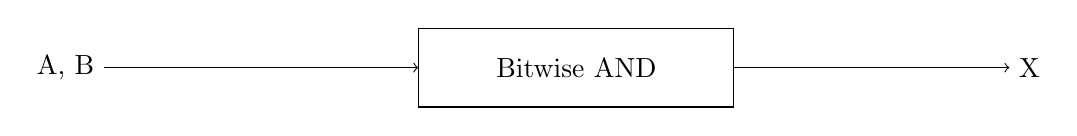
\begin{tikzpicture}
\node[draw,minimum width=4cm,minimum height=1cm] (core) at (0,0) {Bitwise AND};
\draw[->] (-6,0) node[left] {A, B} -- (core.west);
\draw[->] (core.east) -- (5.5,0) node[right] {X};
\end{tikzpicture}
\end{center}
This is a functional port diagram, not a synthesized gate-level schematic.
\subsection{Verilog implementation}
\lstinputlisting[caption={Bitwise AND: module}]{../Verilog/rtl/alu_and.v}
\subsection{Independent unit test}
\lstinputlisting[caption={Bitwise AND: exhaustive unit test}]{../Verilog/tb/tb_and.v}
\subsection{Observed waveform}
\noindent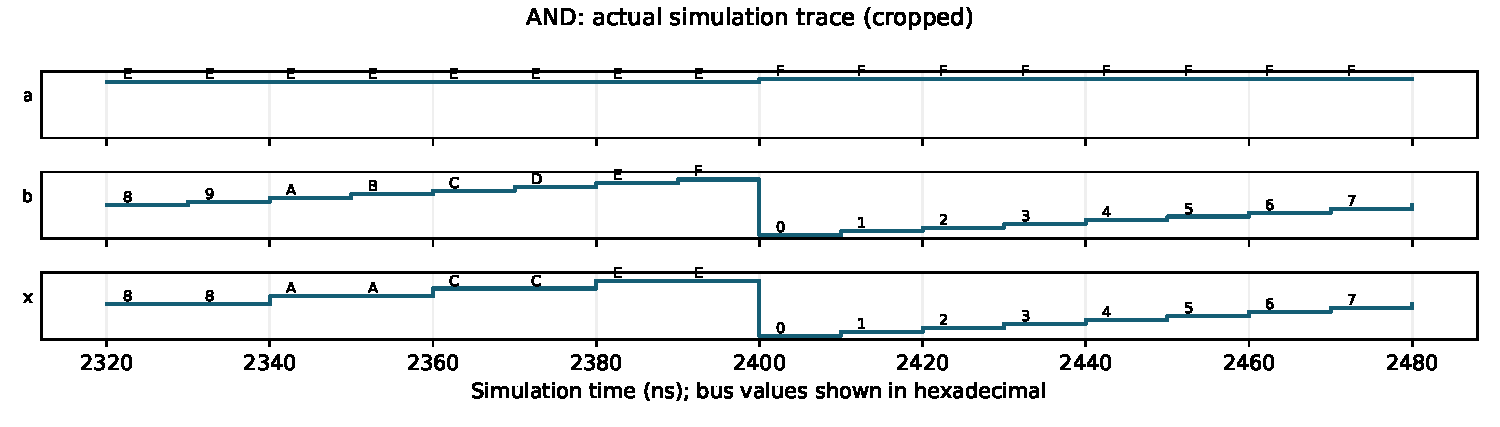
\includegraphics[width=\linewidth]{figures/and.pdf}\par
The crop sweeps B while A=E. Each displayed output follows the per-bit truth table; the testbench checks the full input space beyond this crop.

\clearpage
\section{Bitwise NAND}
$X_i=\neg(A_i\land B_i)$. This complements AND independently for each bit.

\subsection{Functional circuit diagram}
\begin{center}
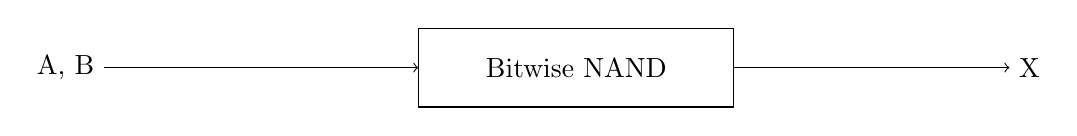
\begin{tikzpicture}
\node[draw,minimum width=4cm,minimum height=1cm] (core) at (0,0) {Bitwise NAND};
\draw[->] (-6,0) node[left] {A, B} -- (core.west);
\draw[->] (core.east) -- (5.5,0) node[right] {X};
\end{tikzpicture}
\end{center}
This is a functional port diagram, not a synthesized gate-level schematic.
\subsection{Verilog implementation}
\lstinputlisting[caption={Bitwise NAND: module}]{../Verilog/rtl/alu_nand.v}
\subsection{Independent unit test}
\lstinputlisting[caption={Bitwise NAND: exhaustive unit test}]{../Verilog/tb/tb_nand.v}
\subsection{Observed waveform}
\noindent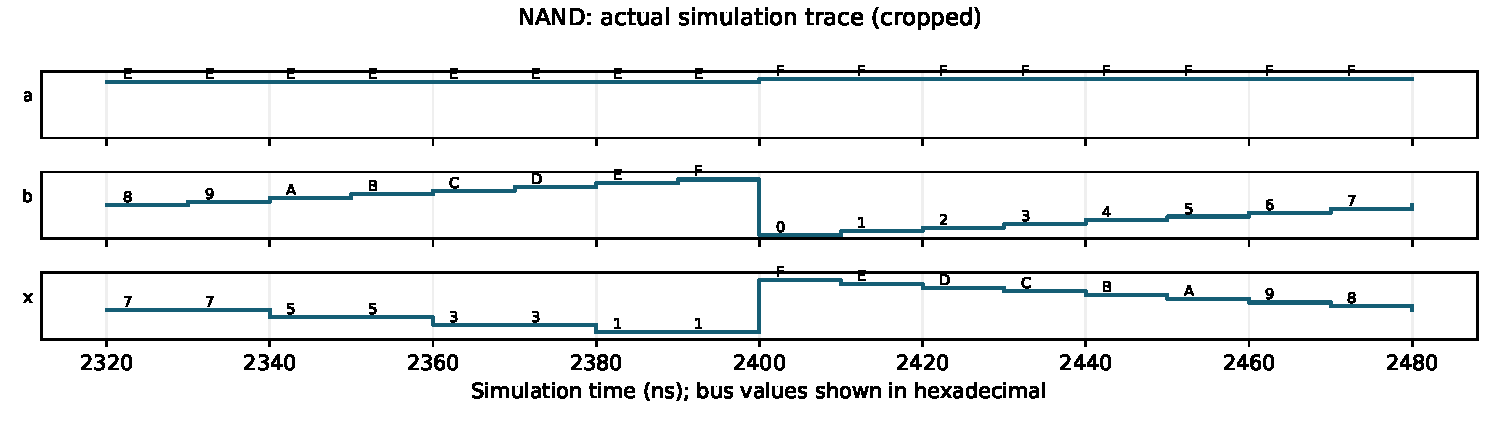
\includegraphics[width=\linewidth]{figures/nand.pdf}\par
The crop sweeps B while A=E. Each displayed output follows the per-bit truth table; the testbench checks the full input space beyond this crop.

\clearpage
\section{Bitwise OR}
$X_i=A_i\lor B_i$. A bit is one when at least one input bit is one.

\subsection{Functional circuit diagram}
\begin{center}
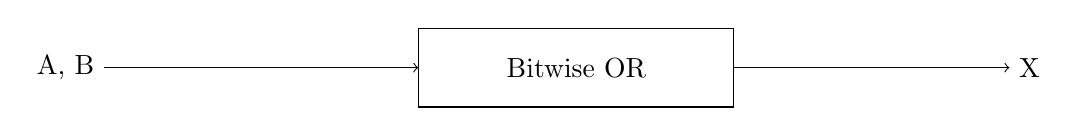
\begin{tikzpicture}
\node[draw,minimum width=4cm,minimum height=1cm] (core) at (0,0) {Bitwise OR};
\draw[->] (-6,0) node[left] {A, B} -- (core.west);
\draw[->] (core.east) -- (5.5,0) node[right] {X};
\end{tikzpicture}
\end{center}
This is a functional port diagram, not a synthesized gate-level schematic.
\subsection{Verilog implementation}
\lstinputlisting[caption={Bitwise OR: module}]{../Verilog/rtl/alu_or.v}
\subsection{Independent unit test}
\lstinputlisting[caption={Bitwise OR: exhaustive unit test}]{../Verilog/tb/tb_or.v}
\subsection{Observed waveform}
\noindent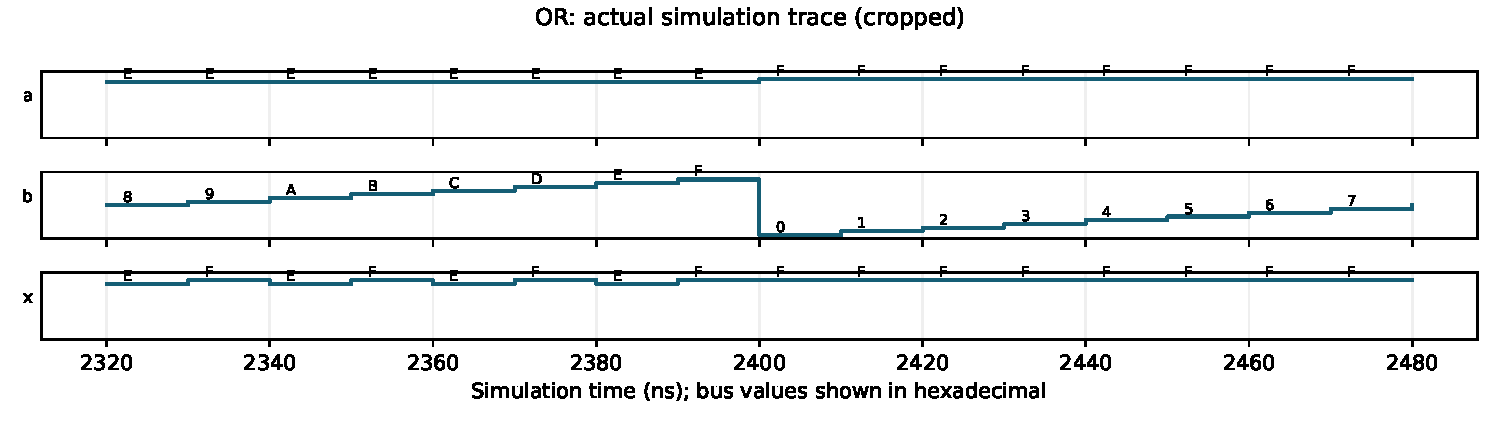
\includegraphics[width=\linewidth]{figures/or.pdf}\par
The crop sweeps B while A=E. Each displayed output follows the per-bit truth table; the testbench checks the full input space beyond this crop.

\clearpage
\section{Bitwise NOR}
$X_i=\neg(A_i\lor B_i)$. A bit is one only when both input bits are zero.

\subsection{Functional circuit diagram}
\begin{center}
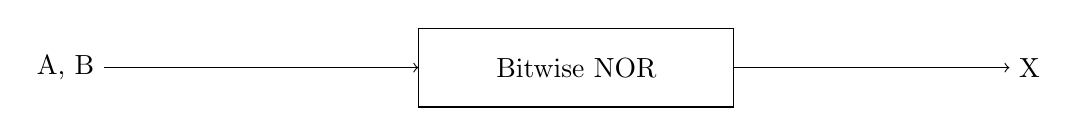
\begin{tikzpicture}
\node[draw,minimum width=4cm,minimum height=1cm] (core) at (0,0) {Bitwise NOR};
\draw[->] (-6,0) node[left] {A, B} -- (core.west);
\draw[->] (core.east) -- (5.5,0) node[right] {X};
\end{tikzpicture}
\end{center}
This is a functional port diagram, not a synthesized gate-level schematic.
\subsection{Verilog implementation}
\lstinputlisting[caption={Bitwise NOR: module}]{../Verilog/rtl/alu_nor.v}
\subsection{Independent unit test}
\lstinputlisting[caption={Bitwise NOR: exhaustive unit test}]{../Verilog/tb/tb_nor.v}
\subsection{Observed waveform}
\noindent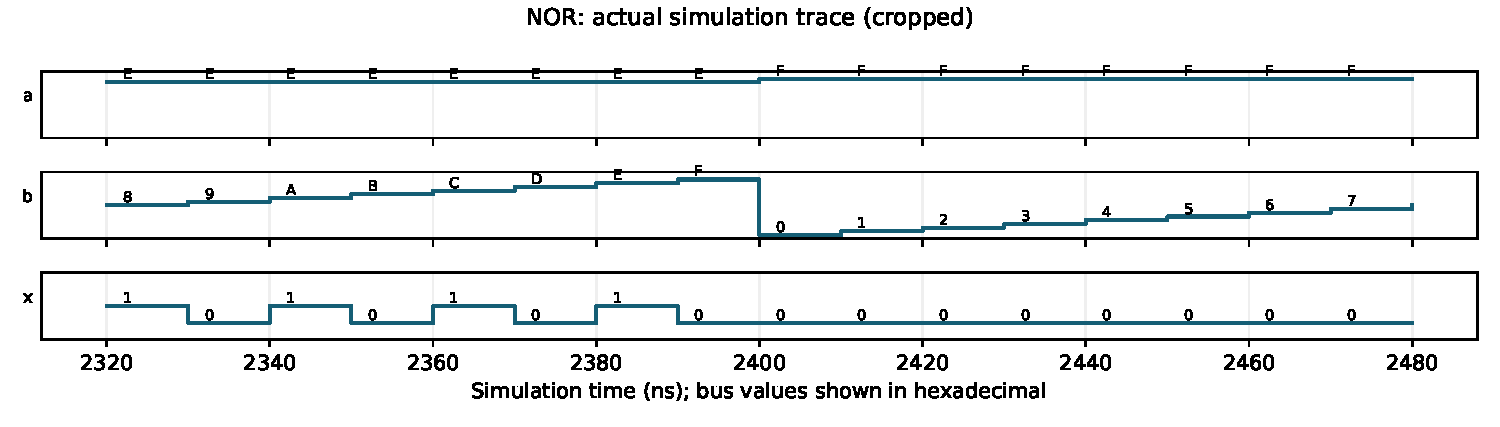
\includegraphics[width=\linewidth]{figures/nor.pdf}\par
The crop sweeps B while A=E. Each displayed output follows the per-bit truth table; the testbench checks the full input space beyond this crop.

\clearpage
\section{Bitwise XOR}
$X_i=A_i\oplus B_i$. Unequal input bits produce one.

\subsection{Functional circuit diagram}
\begin{center}
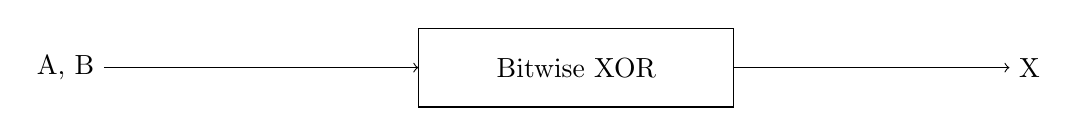
\begin{tikzpicture}
\node[draw,minimum width=4cm,minimum height=1cm] (core) at (0,0) {Bitwise XOR};
\draw[->] (-6,0) node[left] {A, B} -- (core.west);
\draw[->] (core.east) -- (5.5,0) node[right] {X};
\end{tikzpicture}
\end{center}
This is a functional port diagram, not a synthesized gate-level schematic.
\subsection{Verilog implementation}
\lstinputlisting[caption={Bitwise XOR: module}]{../Verilog/rtl/alu_xor.v}
\subsection{Independent unit test}
\lstinputlisting[caption={Bitwise XOR: exhaustive unit test}]{../Verilog/tb/tb_xor.v}
\subsection{Observed waveform}
\noindent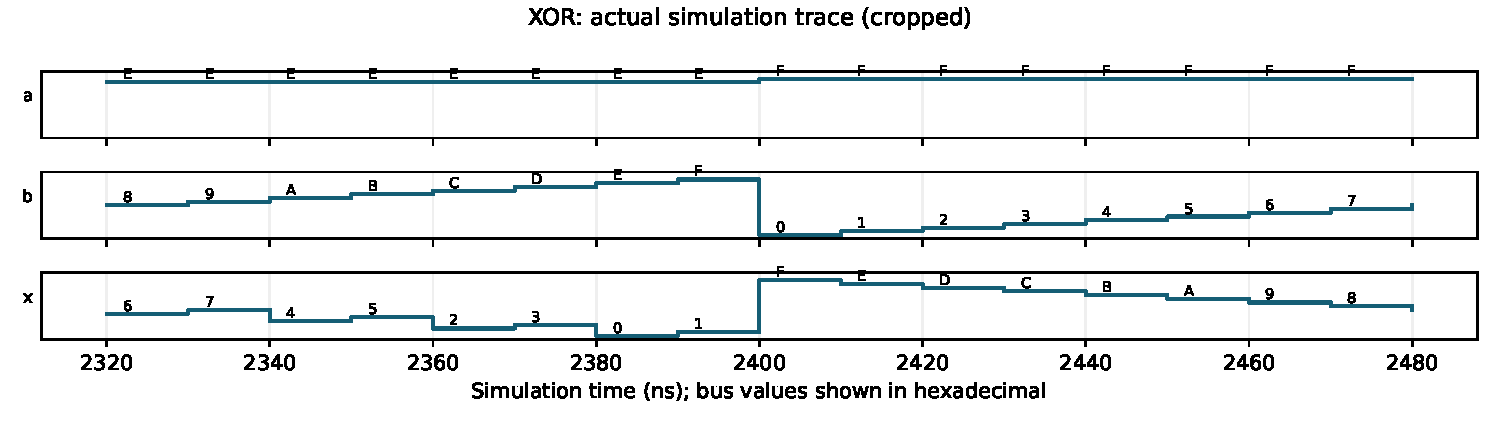
\includegraphics[width=\linewidth]{figures/xor.pdf}\par
The crop sweeps B while A=E. Each displayed output follows the per-bit truth table; the testbench checks the full input space beyond this crop.

\clearpage
\section{Bitwise XNOR}
$X_i=\neg(A_i\oplus B_i)$. Equal input bits produce one.

\subsection{Functional circuit diagram}
\begin{center}
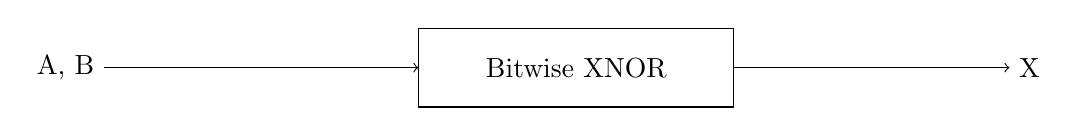
\begin{tikzpicture}
\node[draw,minimum width=4cm,minimum height=1cm] (core) at (0,0) {Bitwise XNOR};
\draw[->] (-6,0) node[left] {A, B} -- (core.west);
\draw[->] (core.east) -- (5.5,0) node[right] {X};
\end{tikzpicture}
\end{center}
This is a functional port diagram, not a synthesized gate-level schematic.
\subsection{Verilog implementation}
\lstinputlisting[caption={Bitwise XNOR: module}]{../Verilog/rtl/alu_xnor.v}
\subsection{Independent unit test}
\lstinputlisting[caption={Bitwise XNOR: exhaustive unit test}]{../Verilog/tb/tb_xnor.v}
\subsection{Observed waveform}
\noindent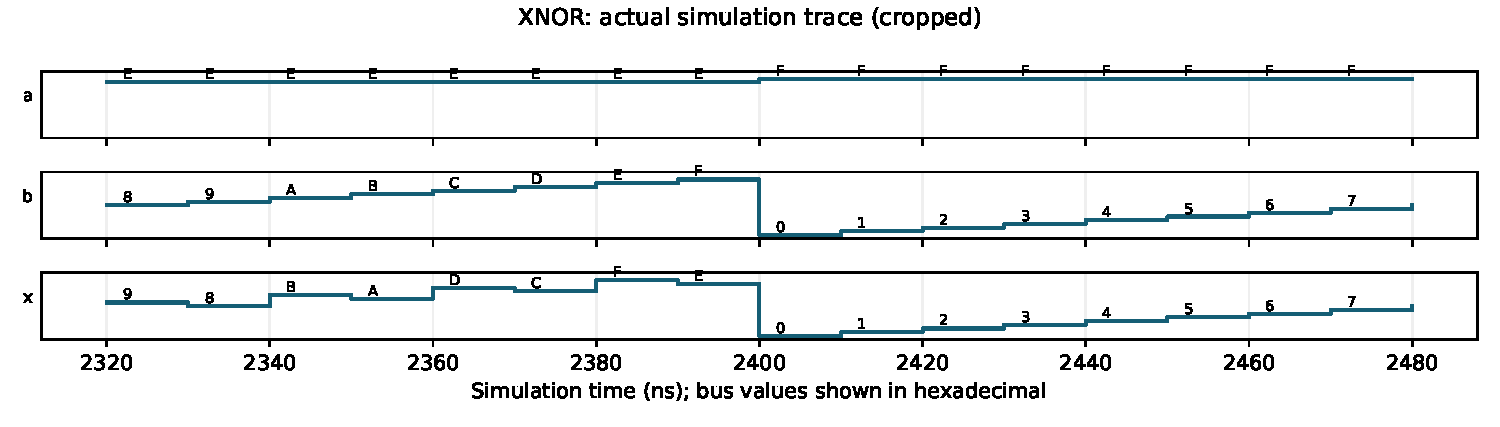
\includegraphics[width=\linewidth]{figures/xnor.pdf}\par
The crop sweeps B while A=E. Each displayed output follows the per-bit truth table; the testbench checks the full input space beyond this crop.

\clearpage
\section{Bitwise NOT}
$X_i=\neg A_i$. This is a unary operation; there is no B port.

\subsection{Functional circuit diagram}
\begin{center}
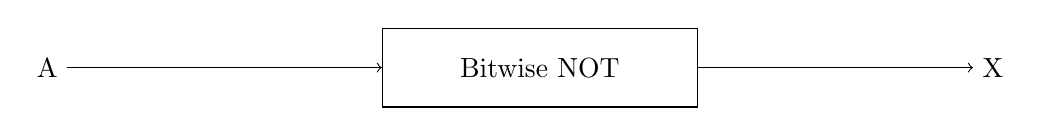
\begin{tikzpicture}
\node[draw,minimum width=4cm,minimum height=1cm] (core) at (0,0) {Bitwise NOT};
\draw[->] (-6,0) node[left] {A} -- (core.west);
\draw[->] (core.east) -- (5.5,0) node[right] {X};
\end{tikzpicture}
\end{center}
This is a functional port diagram, not a synthesized gate-level schematic.
\subsection{Verilog implementation}
\lstinputlisting[caption={Bitwise NOT: module}]{../Verilog/rtl/alu_not.v}
\subsection{Independent unit test}
\lstinputlisting[caption={Bitwise NOT: exhaustive unit test}]{../Verilog/tb/tb_not.v}
\subsection{Observed waveform}
\noindent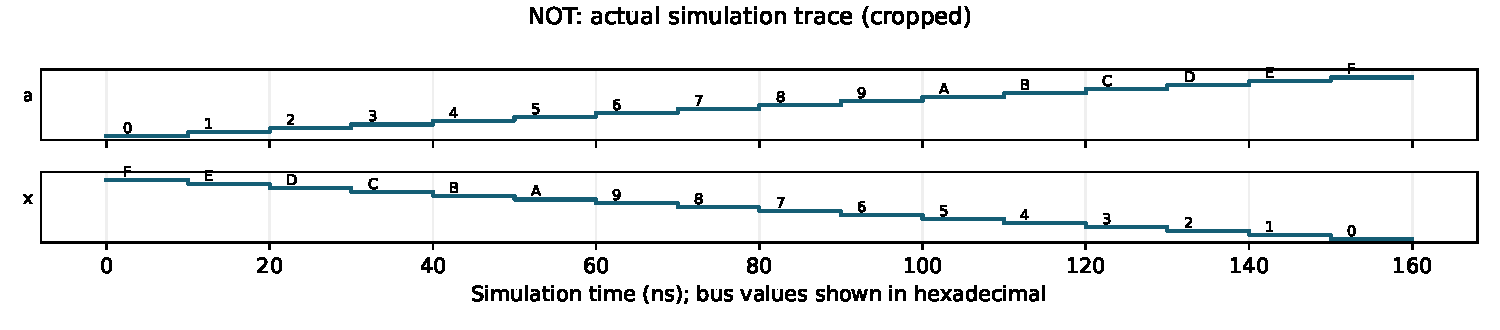
\includegraphics[width=\linewidth]{figures/not.pdf}\par
The trace sweeps every input from hexadecimal 0 through F; X descends from F to 0.

\clearpage
\section{Programmable arithmetic shifter}
The handout defines a programmable fill bit, rather than the automatic sign extension of Verilog's arithmetic-right-shift operator. B[3] selects right (1) or left (0), B[2:1] selects distance 0--3, and B[0] supplies the fill bit. The combinational loop performs up to three one-bit shifts, initializing X to A and Y to zero. Each step captures the departing X bit in Y before replacing it with the fill bit. Left-shift overflow is right-aligned; right-shift overflow is left-aligned. Zero distance preserves A and clears Y. Both assignment examples are covered by exhaustive tests.

For distance $s$ and fill $f$, left shift gives $X=(A2^s+f(2^s-1))\bmod16$, $Y=\lfloor A/2^{4-s}\rfloor$. Right shift gives $X=\lfloor A/2^s\rfloor+f(16-2^{4-s})$, $Y=(A\bmod2^s)2^{4-s}$. These formulas are also the independent test oracle.

\subsection{Functional circuit diagram}
\begin{center}
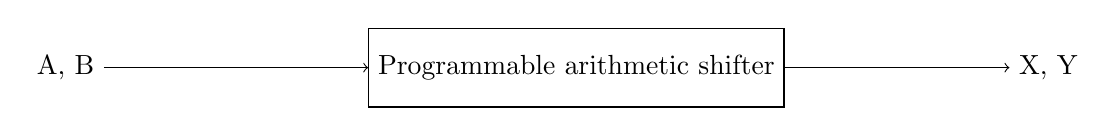
\begin{tikzpicture}
\node[draw,minimum width=4cm,minimum height=1cm] (core) at (0,0) {Programmable arithmetic shifter};
\draw[->] (-6,0) node[left] {A, B} -- (core.west);
\draw[->] (core.east) -- (5.5,0) node[right] {X, Y};
\end{tikzpicture}
\end{center}
This is a functional port diagram, not a synthesized gate-level schematic.
\subsection{Verilog implementation}
\lstinputlisting[caption={Programmable arithmetic shifter: module}]{../Verilog/rtl/alu_shift.v}
\subsection{Independent unit test}
\lstinputlisting[caption={Programmable arithmetic shifter: exhaustive unit test}]{../Verilog/tb/tb_shift.v}
\subsection{Observed waveform}
\noindent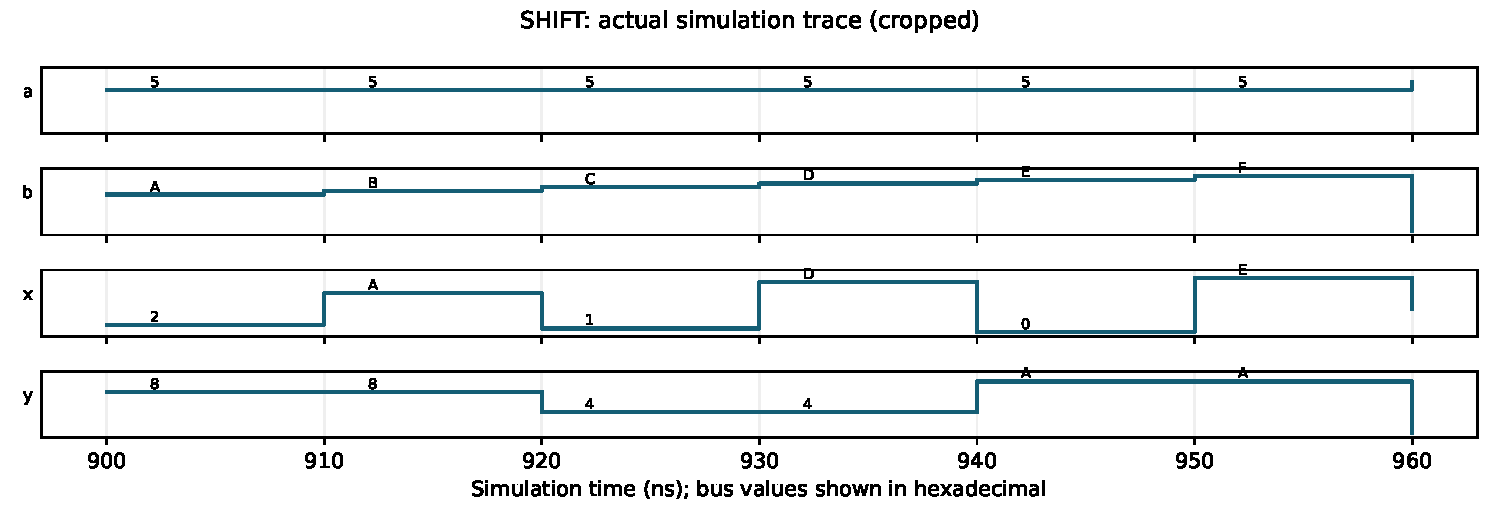
\includegraphics[width=\linewidth]{figures/shift.pdf}\par
At 930 ns, A=5 and B=D give X=D and Y=4, matching the right-shift example. The second crop shows A=B (hexadecimal eleven), B=6, X=8, Y=5 at 1820 ns, matching the left-shift example.
\par\noindent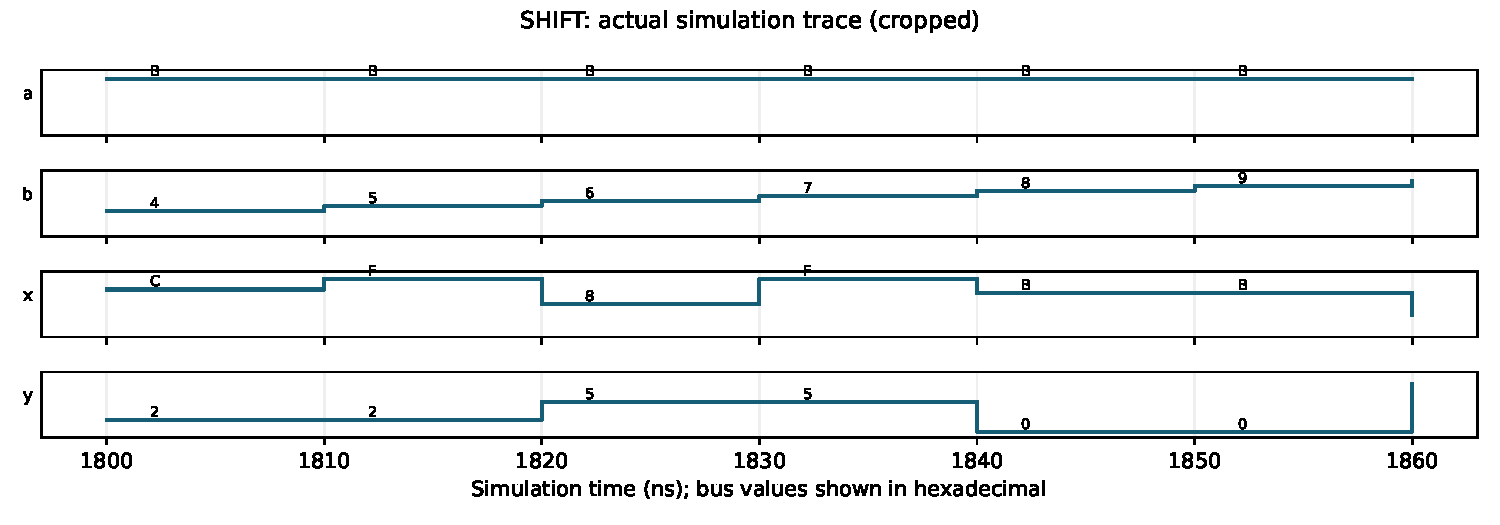
\includegraphics[width=\linewidth]{figures/shift_left.pdf}\par

\clearpage
\section{Unsigned addition with carry}
A five-bit sum preserves the carry: $T=A+B+C_{in}$, $X=T\bmod16$, $C_{out}=\lfloor T/16\rfloor$. Explicit zero extension prevents premature four-bit truncation. For example, $15+15+1=31$ produces X=15 and carry=1. All 512 input combinations are checked.

\subsection{Functional circuit diagram}
\begin{center}
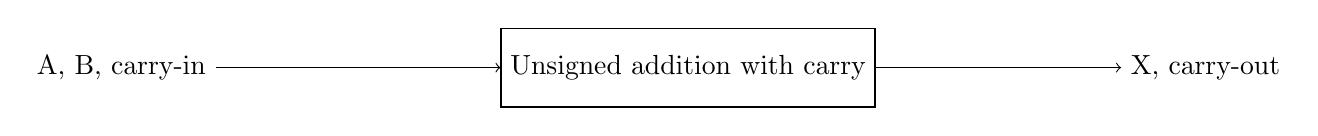
\begin{tikzpicture}
\node[draw,minimum width=4cm,minimum height=1cm] (core) at (0,0) {Unsigned addition with carry};
\draw[->] (-6,0) node[left] {A, B, carry-in} -- (core.west);
\draw[->] (core.east) -- (5.5,0) node[right] {X, carry-out};
\end{tikzpicture}
\end{center}
This is a functional port diagram, not a synthesized gate-level schematic.
\subsection{Verilog implementation}
\lstinputlisting[caption={Unsigned addition with carry: module}]{../Verilog/rtl/alu_add.v}
\subsection{Independent unit test}
\lstinputlisting[caption={Unsigned addition with carry: exhaustive unit test}]{../Verilog/tb/tb_add.v}
\subsection{Observed waveform}
\noindent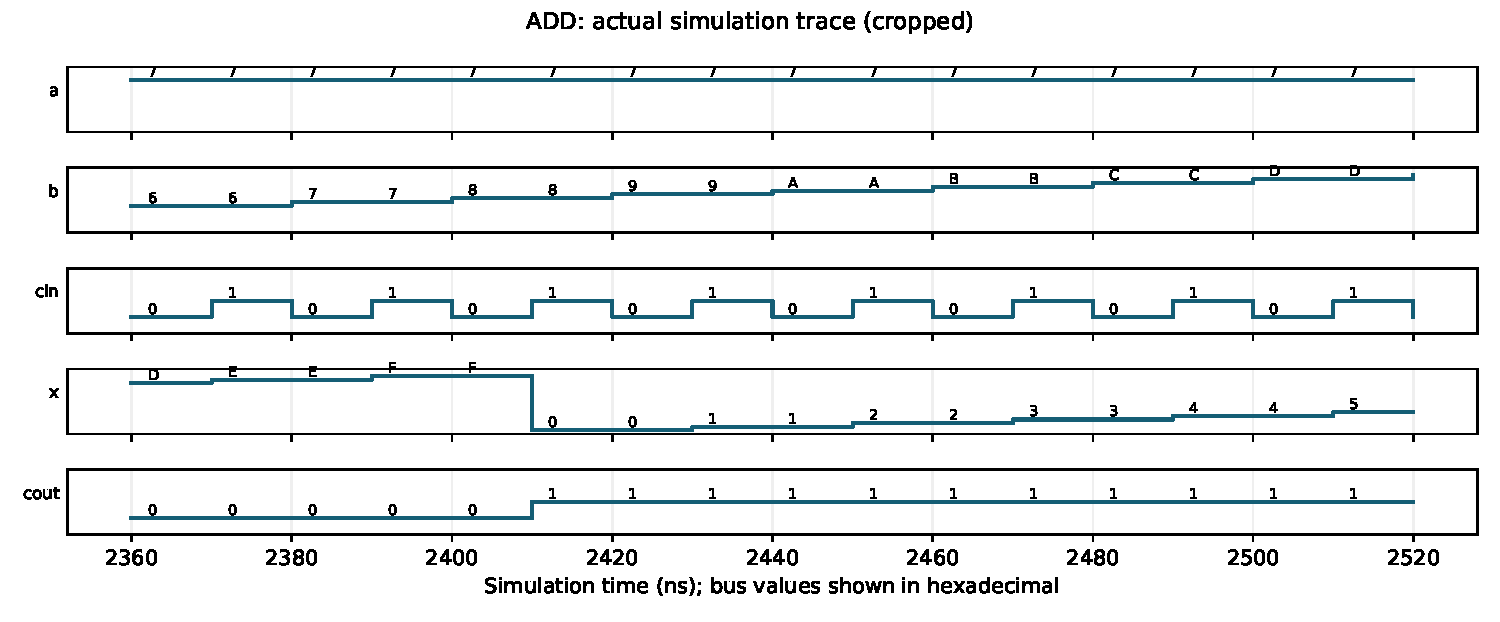
\includegraphics[width=\linewidth]{figures/add.pdf}\par
The crop holds A=7 while B crosses 8: carry-out rises as the five-bit sum reaches sixteen; adjacent samples exercise both carry inputs.

\clearpage
\section{Unsigned subtraction with carry/no-borrow}
The two's-complement adder implements $T=A+\overline{B}+C_{in}$. Consequently, $X=(A-B-(1-C_{in}))\bmod16$. For ordinary subtraction use $C_{in}=1$; use zero to subtract an incoming borrow. $C_{out}=1$ means no unsigned borrow; borrow-out is its complement. For example, $0-1$ with carry-in 1 gives X=15 and carry-out 0. Chaining the carry directly supports multi-nibble subtraction. The bench uses signed integer subtraction and a comparison, not the complemented-adder expression.

\subsection{Functional circuit diagram}
\begin{center}
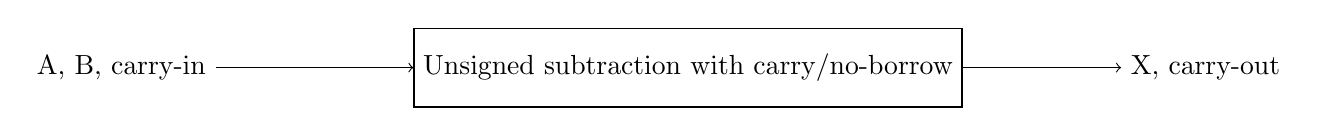
\begin{tikzpicture}
\node[draw,minimum width=4cm,minimum height=1cm] (core) at (0,0) {Unsigned subtraction with carry/no-borrow};
\draw[->] (-6,0) node[left] {A, B, carry-in} -- (core.west);
\draw[->] (core.east) -- (5.5,0) node[right] {X, carry-out};
\end{tikzpicture}
\end{center}
This is a functional port diagram, not a synthesized gate-level schematic.
\subsection{Verilog implementation}
\lstinputlisting[caption={Unsigned subtraction with carry/no-borrow: module}]{../Verilog/rtl/alu_sub.v}
\subsection{Independent unit test}
\lstinputlisting[caption={Unsigned subtraction with carry/no-borrow: exhaustive unit test}]{../Verilog/tb/tb_sub.v}
\subsection{Observed waveform}
\noindent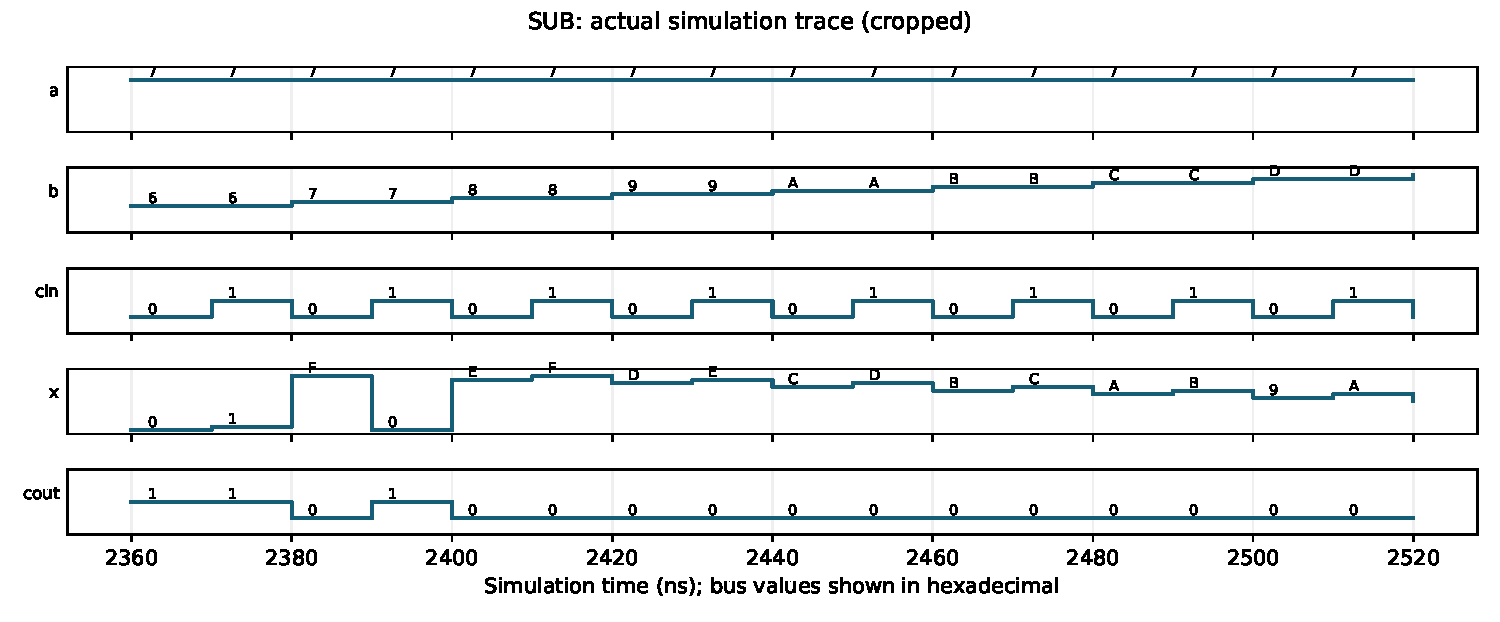
\includegraphics[width=\linewidth]{figures/sub.pdf}\par
The crop holds A=7 while B crosses 7: carry-out distinguishes no borrow from borrow; alternating carry-in values also exercise incoming borrow.

\clearpage
\section{Unsigned multiplication}
The eight-bit product is split into low nibble X and high nibble Y, so $16Y+X=AB$. For example, $15\times15=225$ gives Y=14 and X=1. Both operands are explicitly extended. The test oracle uses repeated addition, independently of the multiplication operator.

\subsection{Functional circuit diagram}
\begin{center}
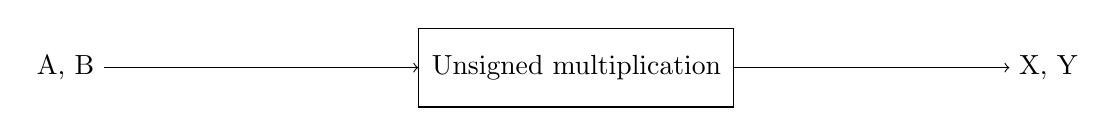
\begin{tikzpicture}
\node[draw,minimum width=4cm,minimum height=1cm] (core) at (0,0) {Unsigned multiplication};
\draw[->] (-6,0) node[left] {A, B} -- (core.west);
\draw[->] (core.east) -- (5.5,0) node[right] {X, Y};
\end{tikzpicture}
\end{center}
This is a functional port diagram, not a synthesized gate-level schematic.
\subsection{Verilog implementation}
\lstinputlisting[caption={Unsigned multiplication: module}]{../Verilog/rtl/alu_mul.v}
\subsection{Independent unit test}
\lstinputlisting[caption={Unsigned multiplication: exhaustive unit test}]{../Verilog/tb/tb_mul.v}
\subsection{Observed waveform}
\noindent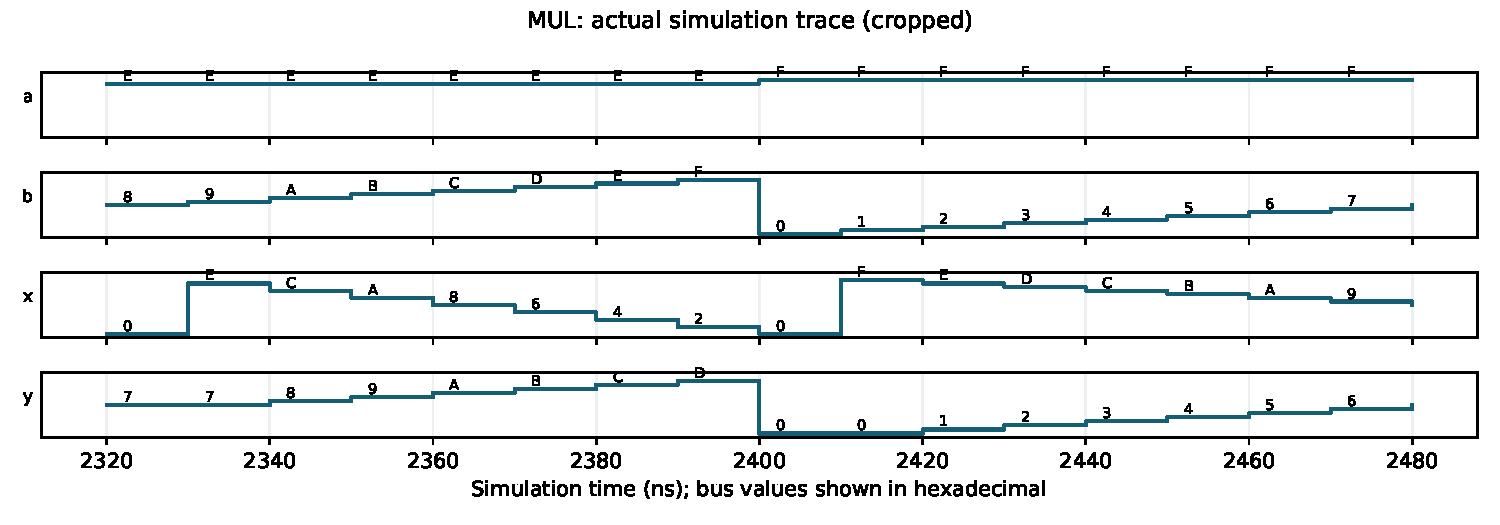
\includegraphics[width=\linewidth]{figures/mul.pdf}\par
With A=E, increasing B changes both product nibbles. For B=F the product is D2, so Y=D and X=2.

\clearpage
\section{Unsigned division and remainder}
For nonzero B, X is the integer quotient and Y is the remainder: $A=BX+Y$ and $0\leq Y<B$. The test oracle uses repeated subtraction. All 240 valid pairs and all 16 zero-divisor pairs are exercised. For B=0, the explicit divide\_by\_zero output is asserted, X=15, and Y=A. These deterministic sentinel values are not a mathematical quotient and remainder and must be interpreted with the error flag. The handout does not prescribe zero-divisor behavior; this is a documented interface choice.

\subsection{Functional circuit diagram}
\begin{center}
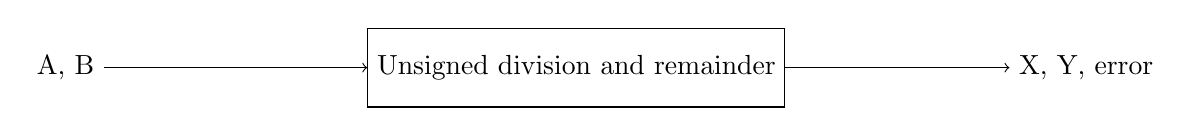
\begin{tikzpicture}
\node[draw,minimum width=4cm,minimum height=1cm] (core) at (0,0) {Unsigned division and remainder};
\draw[->] (-6,0) node[left] {A, B} -- (core.west);
\draw[->] (core.east) -- (5.5,0) node[right] {X, Y, error};
\end{tikzpicture}
\end{center}
This is a functional port diagram, not a synthesized gate-level schematic.
\subsection{Verilog implementation}
\lstinputlisting[caption={Unsigned division and remainder: module}]{../Verilog/rtl/alu_div.v}
\subsection{Independent unit test}
\lstinputlisting[caption={Unsigned division and remainder: exhaustive unit test}]{../Verilog/tb/tb_div.v}
\subsection{Observed waveform}
\noindent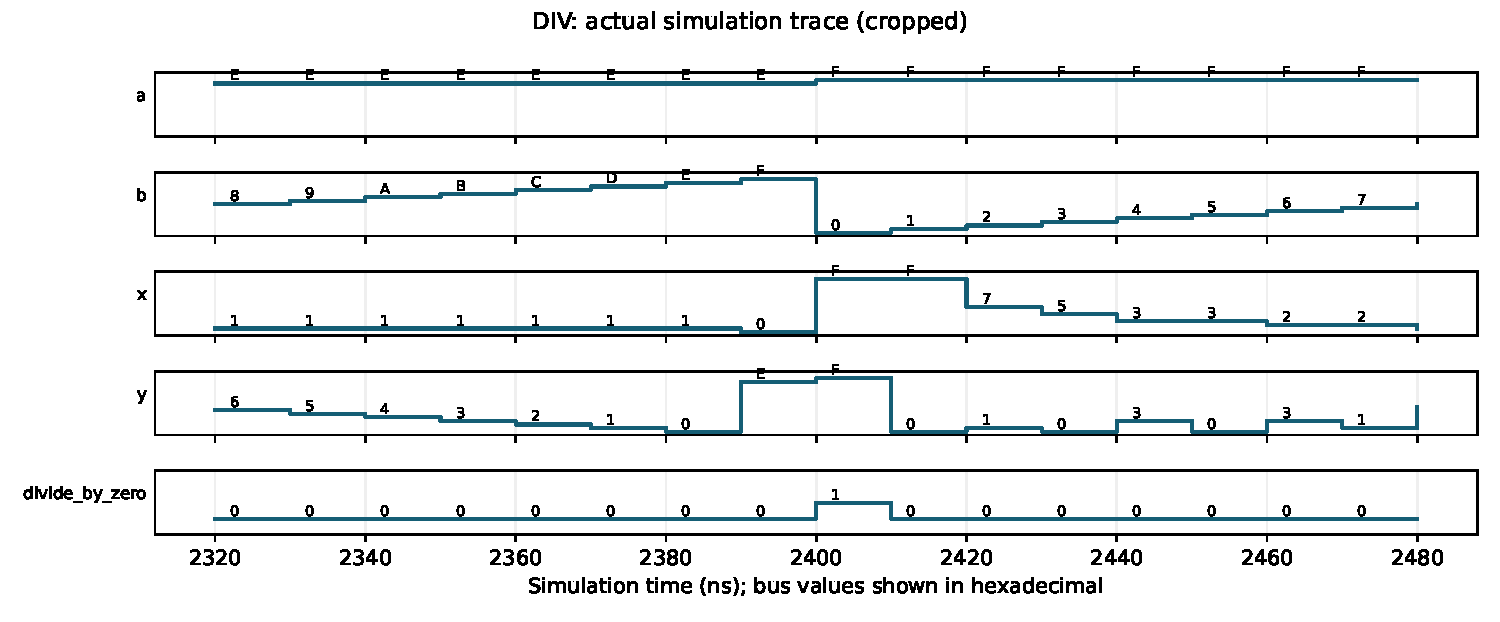
\includegraphics[width=\linewidth]{figures/div.pdf}\par
The crop includes A=F, B=0 at 2400 ns: error rises, X=F, Y=F. For nonzero B, X and Y return to quotient and remainder.

\clearpage
\section{Reproducing the results}
From the repository root, run the commands below. Icarus Verilog, Python 3 with Matplotlib, and a LaTeX installation with listings, graphics, and TikZ are required. The test runner also recognizes the local Icarus installation prepared in this cloud environment. No server or credentials are required.
\begin{lstlisting}[language=bash,caption={Reproduce simulations and report}]
bash scripts/test.sh
python scripts/render_waveforms.py
python scripts/build_report.py
cd latex
pdflatex -interaction=nonstopmode -halt-on-error report.tex
pdflatex -interaction=nonstopmode -halt-on-error report.tex
\end{lstlisting}
RTL and unit benches are in the Verilog folder. Raw traces and per-unit test logs are generated in build. The report source and vector waveform figures are in latex. The companion archive contains the PDF, source folders, and scripts. Replace the identity placeholders and rebuild the report before naming the archive GroupName-ProjectStep2.zip. Review the implementation and explanations, and adapt this standalone layout to the course template if required.

\section{Conclusion}
The twelve separate four-bit functions passed exhaustive functional simulation. The two shift examples agree with the assignment, arithmetic outputs preserve carry, high-product bits, and division remainders, and zero-divisor behavior is explicit. The main design ambiguities were overflow alignment in the shifter and the carry convention for subtraction; these were resolved through the supplied examples and a documented no-borrow interface. Independent reference models and full input enumeration make the results stronger than a few selected demonstrations. The next project step can instantiate these modules beneath an opcode controller without merging their implementations. Physical synthesis and optional wider datapaths remain separate work.
\end{document}
